\section{Method}
\label{section:Method}

\begin{figure}[b]
	\centering
	%\fcolorbox{bordercolor}{paddingcolor}{image}
	\fcolorbox{red}{red}{\includegraphics[width=0.2\linewidth]{ex2.png}}
	\fcolorbox{green}{green}{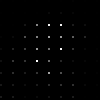
\includegraphics[width=0.2\linewidth]{deltaPulses_ex2_big.png}}
	\fcolorbox{cyan}{cyan}{
\includegraphics[width=0.2\linewidth]{rectPulses_ex2.png}}
	\fcolorbox{blue}{blue}{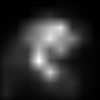
\includegraphics[width=0.2\linewidth]{trianglePulses_ex2.png}}
	
	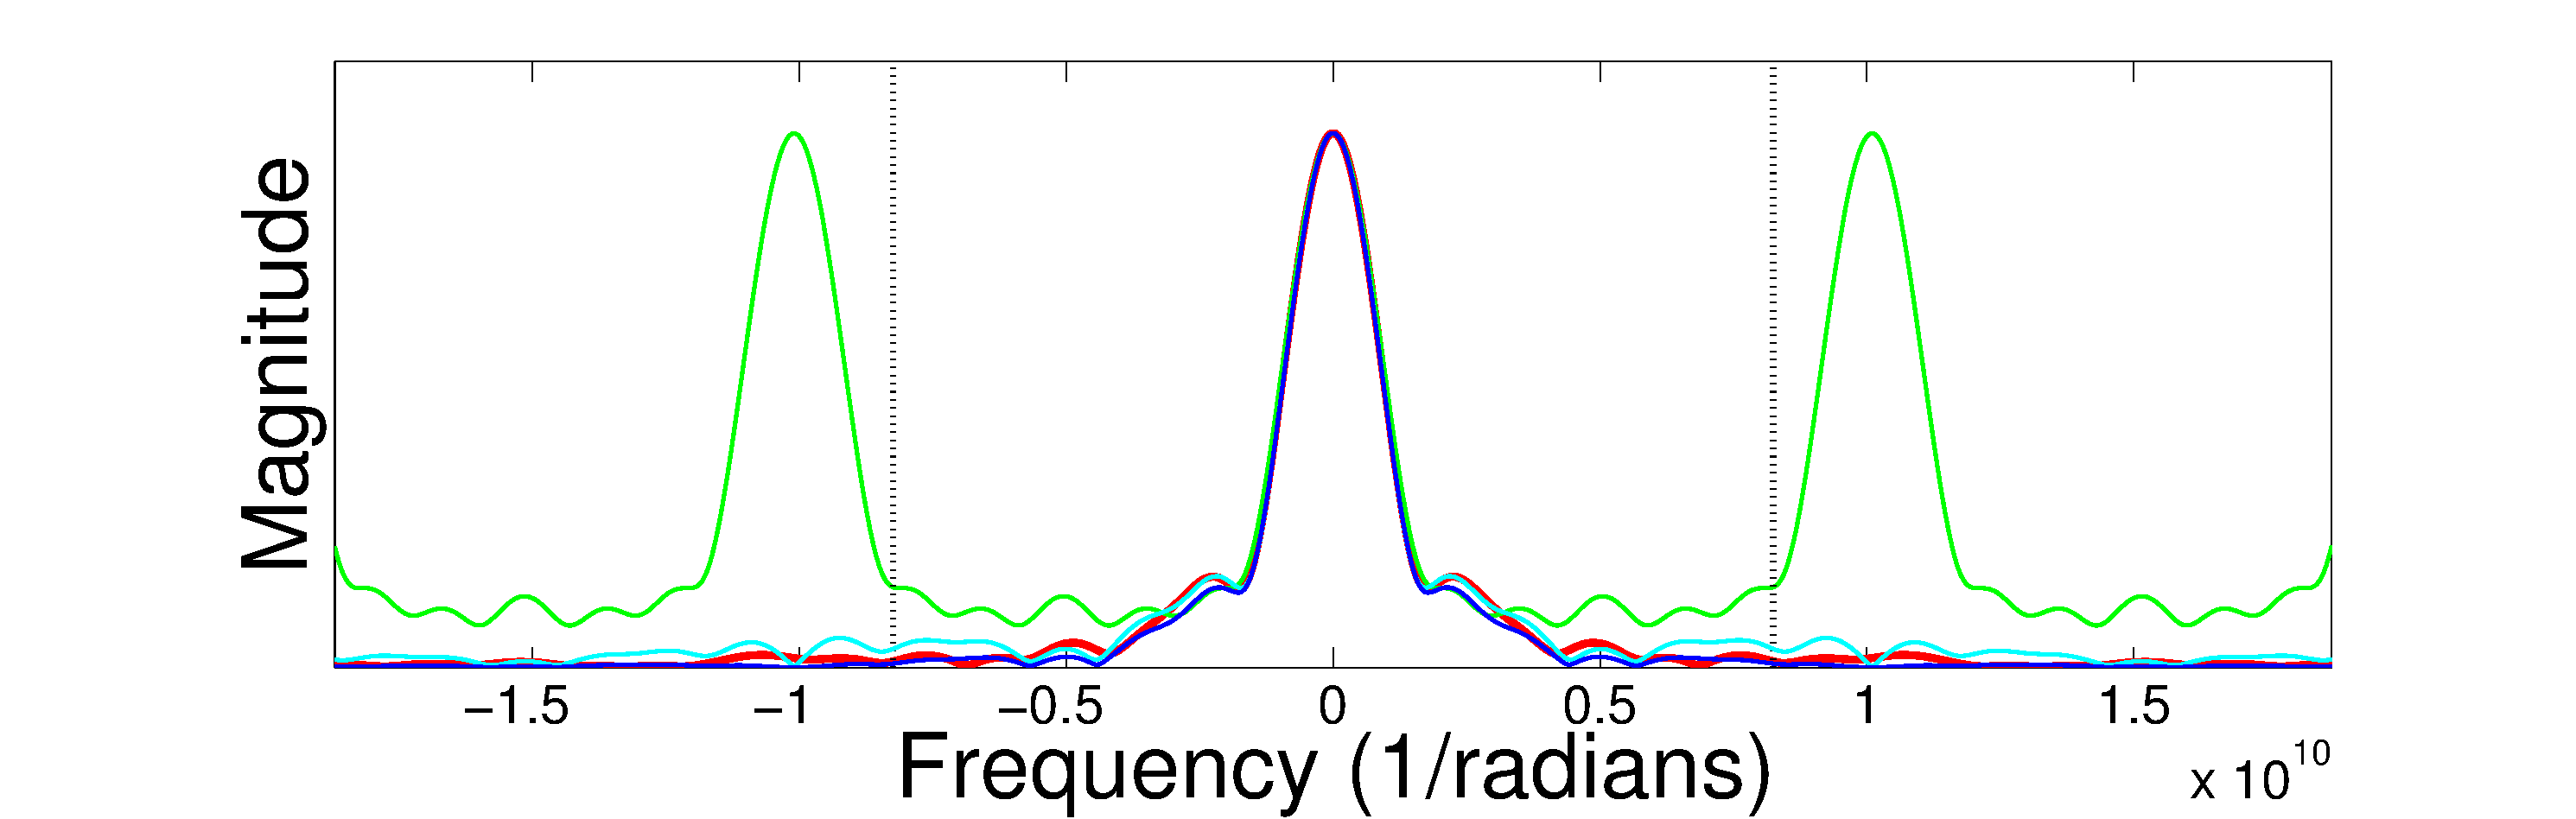
\includegraphics[width=0.95\linewidth]{freqfig_9pulses_wrect_zoom_ex2_2.pdf}
	\caption{\footnotesize{Accurately modeling the frequencies of an image is crucial for fitting VLBI measurements during image reconstruction. Here we show, that with the same number of parameters, we can much more accurately model the true frequency distribution. A slice of frequencies for the true image is shown in red. Overlayed we show the effect of using the traditional discretized imaging model (green), and our improved model for rectangle (cyan) and triangle (blue) pulses. The dotted lines denote the frequency range sampled in Fig~\ref{fig:uvcov}b. Representing an image in this way reduces modeling errors for higher frequencies during image reconstruction.}}
	\label{fig:pulses}
\end{figure}

			
%In this section we describe our proposed algorithm for reconstructing an image using bispectrum measurements.
% obtained using a VLBI telescope array. 
Reconstructing an image using bispectrum measurements is an ill-posed problem, and as such there are an infinite number of possible images that explain the data~\cite{rusenimaging}. 
%To find an optimal solution, we must rely on prior assumptions about the ``visual" universe. 
The challenge is to find an explanation that respects our prior assumptions about the ``visual" universe
%looks  ``good" under some measure
while still satisfying the observed data. 
%Note that this problem differs from traditional sparse spectral reconstruction methods (e.g MRI, CT) due to the large atmospheric phase errors. 


%For every two telescopes in an $N$ telescope array we measure a single complex Fourier component of $I_{\lambda}$. Assuming that the atmosphere does not affect our measurements, this means that we have constraints on $ \frac{N(N-1)}{2} $ of the image's frequency components. The task of reconstructing an image from just these components is highly under-constrained since there are infinite possibilities for what values could fill the remaining frequency components. Therefore, to find an optimal solution, we must rely on our prior assumptions about the ``visual" universe. Using a prior image model narrows our search space substantially and helps us find a reasonable looking image that also fits the the measurements~\cite{felli1989very}. 


\subsection{Continuous Image Representation}


The image that we wish to recover, $I_{\lambda}(\ell,m)$, is defined over the continuous space of angular coordinates $l$ and $m$. 
%However, computers require that we work with discrete elements.  
%rather than discretizing the measurements, 
%\katie{To account for the expected resolution of the instrument,} 
Many algorithms assume a discretized image of point sources during reconstruction 
%and subsequently blur the final image to account for the expected instrumental resolution
~\cite{taylor1999synthesis}. This discretization introduces errors during the reconstruction optimization, especially in fitting the higher frequency visibilities.
Instead, we parameterize a continuous image using a discrete number of terms. 
{\it This parameterization not only allows us to model our emission with a continuous image, but it also reduces modeling errors during optimization. }
%{\it This parameterization not only allows us to reduce modeling error} by easily evaluating the likelihood of measuring a set of visibilities from an estimate of the continuous image during optimization. 

Since each measured complex visibility is approximated as the Fourier transform of $I_{\lambda}(\ell,m)$, a convenient parameterization of the image is to represent it as a discrete number of scaled and shifted continuous pulse functions, such as triangular pulses.
% that have an analytic Fourier transform. 
For a scene defined in the range $\ell \in [-\frac{F_\ell}{2}, \frac{F_\ell}{2}]$ and $m \in [-\frac{F_m}{2}, \frac{F_m}{2}]$,
%and is assumed to have zero flux density outside the field of view,
we parameterize our space into $N_\ell \times N_m$ scaled pulse functions, $h(l,m)$, centered around 

%\vspace{-.17in}

\begin{align}
 l &= i \Delta_{\ell} + \frac{\Delta_{\ell}}{2}  -\frac{F_\ell}{2} \hspace{0.26in} \mbox{for} \hspace{0.1 in} i = 0,...,N_\ell-1
 \label{eq:discrete1}
\\m &= j\Delta_m + \frac{\Delta_m}{2} -\frac{F_m}{2} \hspace{0.1in} \mbox{for} \hspace{0.1 in} j= 0,...,N_m-1
\label{eq:discrete2}
\end{align} 


\vspace{-.09in}
\noindent{for $\Delta_{\ell} = \frac{F_\ell}{N_\ell}$ and $\Delta_m = \frac{F_m}{N_m}$. Using Eq.~\ref{eq:discrete1} and~\ref{eq:discrete2} we can represent a continuous image as a discrete sum of shifted pulse functions scaled by $x[i,j]$. We refer to this image as $\hat{I}_{\lambda}({\bf x})$ for vectorized coefficients ${\bf x}$. 


%
%\begin{figure}[b]
%	\centering
%	%\fcolorbox{bordercolor}{paddingcolor}{image}
%	\fcolorbox{red}{red}{\includegraphics[width=0.2\linewidth]{images/newfigscvpr/pulses/ex2.png}}
%	\fcolorbox{green}{green}{\includegraphics[width=0.2\linewidth]{images/newfigscvpr/pulses/deltaPulses_ex3.png}}
%	\fcolorbox{cyan}{cyan}{
\includegraphics[width=0.2\linewidth]{images/newfigscvpr/pulses/rectPulses_ex2.png}}
%	\fcolorbox{blue}{blue}{\includegraphics[width=0.2\linewidth]{images/newfigscvpr/pulses/trianglePulses_ex3.png}}
%	
%	\includegraphics[width=0.95\linewidth]{images/newfigscvpr/pulses/freqfig_8pulses_wrect_zoom_ex3.eps}
%	\caption{\footnotesize{To accuratetly model an image's visibilities, we must write {\color{red} BLAH BLAH BLAH. TODO THIS CAPTION} Representing an image in this way reduces modeling errors during image reconstruction.}}
%	\label{fig:pulses}
%\end{figure}





%\begin{figure}[b]
%	\centering
%	%\fcolorbox{bordercolor}{paddingcolor}{image}
%	\fcolorbox{red}{red}{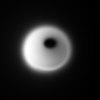
\includegraphics[width=0.2\linewidth]{images/newfigscvpr/newresults/blackhole40/blackhole40.png}}
%	\fcolorbox{green}{green}{\includegraphics[width=0.2\linewidth]{images/newfigscvpr/pulses/deltaPulses.png}}
%	\fcolorbox{cyan}{cyan}{\includegraphics[width=0.2\linewidth]{images/newfigscvpr/pulses/rectPulses.png}}
%	\fcolorbox{blue}{blue}{\includegraphics[width=0.2\linewidth]{images/newfigscvpr/pulses/trianglePulses.png}}
%	
%	\includegraphics[width=0.95\linewidth]{images/newfigscvpr/pulses/freqfig_8pulses_wrect_zoom.eps}
%	\caption{\footnotesize{To accuratetly model an image's visibilities, we must write {\color{red} BLAH BLAH BLAH. TODO THIS CAPTION} Representing an image in this way reduces modeling errors during image reconstruction.}}
%	\label{fig:pulses}
%\end{figure}

%
%   \begin{figure}[ht!]
%\centering
%  {\includegraphics[width=\linewidth]
%                   {images/forwardmodel/trianglePulse.eps}}                                               
%                    \caption{\footnotesize{An example of a continuous 1D image defined in terms of 1D triangle pulses. Pulses are shifted and scaled by a discrete set of values, $X[i]$. These shifted and scaled pulses are then summed together to make a single continuous image. In this example $X[i] = [1,2,3,1,1,4]$. Note how each point in the continuous image is a linear interpolation of its neighbors when using a triangle pulse. Representing an image in this way reduces modeling errors during image reconstruction. }}
% \label{fig:trianglePulse}
%\end{figure}

%\begin{align*}
%I_{\lambda}(\ell,m) \approx \sum_{i=0}^{N_{\ell}-1}{\sum_{j=0}^{N_m-1} X[i,j] h \left(l- \left( \Delta_{\ell}i + \frac{\Delta_{\ell}}{2} + a_{\ell} \right),m- \left( \Delta_mj + \frac{\Delta_m}{2} + a_m \right)\right) }
%\label{eq:discrete}
% \end{align*} 
 
 Due to the shift theorem~\cite{oppenheim1997signals}, plugging this image representation into the van Cittert-Zernike theorem (Eq.~\ref{eq:visibility}) results in a closed-form solution to the visibilities in terms of $H(u,v)$, the Fourier transform of $h(l,m)$, as seen in Eq.~\ref{eq:formodel}. Note that performing a continuous integration has been reduced to a linear matrix operation similar to a Discrete Time Fourier Transform (DTFT). 

\begin{align}
		 \Gamma(u,v) &\approx \int_{- \infty}^{\infty}\int_{- \infty}^{\infty} {e^{-i 2 \pi  (u\ell + vm) }} 
		 \nonumber \\ & \quad \sum_{i=0}^{N_\ell-1}\sum_{j=0}^{N_m-1} x[i,j] 
		h \biggl(\ell- \bigl( \Delta_{\ell}i + \frac{\Delta_{\ell}}{2}  -\frac{FOV_\ell}{2} \bigr), \nonumber\\ 
		&  \qquad \qquad \qquad m- \bigl( \Delta_mj + \frac{\Delta_m}{2} -\frac{FOV_m}{2} \bigr) \biggl)  d\ell dm  
		\nonumber\\ &=  \sum_{i=0}^{N_\ell-1}{\sum_{j=0}^{N_m-1}  x[i,j] e^{-i 2 \pi \left(u  \left( \Delta_{\ell}i + \frac{\Delta_{\ell}}{2} + a_\ell \right) + v \left( \Delta_mj + \frac{\Delta_m}{2} + a_m \right)  \right)} H(u, v)} \nonumber\\ & = A {\bf x} = \left( A^{\Re} + i A^{\Im} \right) {\bf x}
		\label{eq:formodel}
		\end{align}

 
In Figure~\ref{fig:pulses} we show that this representation allows us to approximate the true frequency components more accurately than a discretized set of point sources, especially for high frequencies.  
%In optimization, this formulation asks us to find the best set of coefficients $X[i,j]$ to explain $I_{\lambda}(\ell, m)$ under the assumed pulse model. 
Any pulse with a continuous closed-form Fourier transform can be used in this representation (e.g. rectangle, triangle, sinc, Gaussian). The chosen pulse places an implicit prior on the reconstruction. For instance, a sinc pulse with frequency and spacing $\Delta$ can reconstruct any signal with a bandwidth less than $\frac{\Delta}{2}$~\cite{oppenheim1997signals}. In this work we choose to use a triangle pulse with width $(2\Delta_\ell, 2\Delta_m)$ since this is equivalent to linearly interpolating between pulse centers and also simplifies 
%lends itself nicely to
non-negativity constraints. %(Figure~\ref{fig:trianglePulse}). 
Although we developed this image model for VLBI image reconstruction, it has potential applicability to a much more general class of imaging problems that rely on frequency constraints.
% - such as magnetic resonance imaging (MRI)~\cite{lustig2007sparse}. 

%Many algorithms, such as CLEAN, circumvent this by quantizing the measured frequencies so that they lie on the DFT components of a discrete sized image - a process known as ``gridding". 
%Although there has been a fair amount of work on developing a gridding function~\cite{thompson2008interferometry}, this process always introduces errors that are difficult to account for. 


%\subsection{Bispectrum Gridding}
%
%The number of bispectrum values grows combinatorially with the number of telescopes. While this does not pose a problem when the number of telescopes is small, as is the case with the EHT, it can make optimization very slow and memory intensive for larger interferometers. For instance, The Atacama Large Millimeter/submillimeter Array (ALMA) consits of 66 telescopes spanning 16 km. Although atmospheric effects are not as detrimental to visibilities from these shorter baselines, they still need to be removed through calibration. While a single timestep from the 8-telescope EHT array results in at most 56 bispectrum values, ALMA's 66 telescopes results in 45,760 bispectrum values. 
%
%To make reconstruction more managable for large arrays we extend an idea called {\it gridding} from visibility to bispectrum data. In gridding, visiblity values at selected $(u,v)$ points are assigned based upon observed values. These new data points can then be used to constrain the image reconstruction. 
%%Traditionally, $(u,v)$ values corresponding to the DFT grid are chosen so that an inverse DFT can be used to generate an image; however, in reality these methods do not require sampling on regular grids. 
%We define a 2D multivariate Gaussian distribution, $\mathcal{N}(\cdot,\cdot)$, over the real ($\Re$) and imaginary ($\Im$) components of each point in the bispectrum space, $B$, as
%
%{
%	\begin{align}
%	\notag & B(u_1,v_1,u_2,v_2,u_3,v_3) \\
%	 & \sim \mathcal{N}( \Gamma (u_1,v_1)  \Gamma (u_2,v_2)  \Gamma (u_3,v_3) , \Sigma_{u_1,v_1,u_2,v_2,u_3,v_3}).
%	% \\ & = \mathcal{N} \left( \Spvek{ \Re \left[ \Gamma (u_1,v_1)  \Gamma (u_2,v_2)  \Gamma (u_3,v_3) \right]; \Im \left[ \Gamma (u_1,v_1)  \Gamma (u_2,v_2)  \Gamma (u_3,v_3) \right] }, \Spvek{\sigma^{\Re,\Re} \hspace{0.1in} \sigma^{\Re, \Im}; \sigma^{\Re, \Im} \hspace{0.1in} \sigma^{\Im, \Im}} \right)
%	%& \hspace{20mm} \forall \hspace{3mm} i,j,k \in [1,N] \hspace{5mm} s.t \hspace{5mm} i<j<k
%	\end{align}
%}
%
%%\noindent{Using our measured visibilities, we can estimate the distribution around sample points in this space }
%Using our measured visibilities, we sample points in this space. 
%
%{\footnotesize
%	\begin{align}
%	\notag b(u_1, v_1, u_2, v_2, u_3,v_3) & = b(\mathbf{p}) \\
%	 & = \Gamma_{i,j}^{meas}(u_1,v_1) \Gamma_{j,k}^{meas}(u_2,v_2) \Gamma_{k,i}^{meas}(u_3,v_3) 
%	\end{align}
%}
%
%\noindent{where $u_3 = -u_1-u_2$, $v_3 = -v_1-v_2$, and each set of 3 independent $\Gamma$s are measured concurently using telescopes $i,j$ and $k$. For notational purposes, we let $\mathbf{p} = [u_1, v_1, u_2, v_2, u_3, v_3]$ and use the notation $\mathbf{p}_k$ to denote the $k^{th}$ entry into the vector, e.g. $\mathbf{p}_1 = u_1, \mathbf{p}_3 = u_2$.}
%
%Although the error due to atmospheric inhomogeneity cancels when using the bispectrum, residual error exists due to thermal noise and fluctuations in each telescope's gain~\cite{thompson2008interferometry}. This introduces Gaussian noise on each complex visibility measurement, $\Sigma_{i,j}$ for telescopes $i$ and $j$. Since the bispectrum is the product of three visibilities, its noise distribution is not Gaussian; nonetheless, its noise is dominated by a Gaussian bounding its first-order noise terms. In the appendix  we show evidence to suggest that this is a reasonable approximation.
%
%{\footnotesize
%	\begin{align}
%	%\notag  \Sigma_{u_1,v_1, u_2,v_2, u_3,v_3} & 
%	\notag \Spvek{\sigma_{\mathbf{p}}^{\Re,\Re} \hspace{0.1in} \sigma_{\mathbf{p}}^{\Re, \Im}; \sigma_{\mathbf{p}}^{\Re, \Im} \hspace{0.1in} \sigma_{\mathbf{p}}^{\Im, \Im}} & \approx |\Gamma_{j,k}^{meas}(u_2,v_2) \Gamma_{k,i}^{meas}(u_3,v_3) | \Sigma_{i,j}  \\
%	\notag &  + |\Gamma_{k,i}^{meas}(u_3,v_3) \Gamma_{i,j}^{meas}(u_1,v_1) | \Sigma_{j,k}  \\
%	 &  + |\Gamma_{i,j}^{meas}(u_1,v_1) \Gamma_{j,k}^{meas}(u_2,v_2) | \Sigma_{k,i}
%	%& = \Spvek{\sigma_{u_1,v_1, u_2,v_2, u_3,v_3}^{\Re,\Re} \hspace{0.1in} \sigma_{u_1,v_1, u_2,v_2, u_3,v_3}^{\Re, \Im}; \sigma_{u_1,v_1, u_2,v_2, u_3,v_3}^{\Re, \Im} \hspace{0.1in} \sigma_{u_1,v_1, u_2,v_2, u_3,v_3}^{\Im, \Im}}
%	\end{align}
%}
%
%
%
% Traditional convolutional-gridding methods used for visibities cannot be extended to bispectrum data since the bispectrum sampling function is not separable. Instead, we interpolate the distribution around a selected point given samples from its neighborhood. We can then use the distribution around selected points to constrain image reconstruction. We model the bispectrum space using a Gaussian processes and use regression methods to resample our data at the selected points. 
%%If we assume that the emission is contained within a region of size $FOV_{\ell}\times FOV_m$, then we know that along each $u$ and $v$ dimension $B(u_1,v_1,u_2,v_2,u_3,v_3)$'s signal has a maximum frequency of  $\frac{FOV_{\ell}}{2}$ and $\frac{FOV_{m}}{2}$ respectively. We also know that since our emission image is real, $\Gamma(u,v) = \Gamma^*(-u,-v)$. 
%We use three observations to intelligently sample and interpolate $B$:
%
%\begin{enumerate}
%	\item $I_{\lambda}$ is real, therefore
%	$\mathbf{E} [ B(\mathbf{p})] = \mathbf{E} [ B^*(-\mathbf{p}) ]$ %$\mathbf{E} [ B(u_1,v_1,u_2,v_2,u3,v_3)] = \mathbf{E} [ B^*(-u_1,-v_1,-u_2,-v_2,-u3,-v_3) ]$
%	\item If the emission is contained within a region of size $FOV_{\ell}\times FOV_m$, then $\mathbf{E}[B]$ is a function with a maximum frequency of  $\frac{FOV_{\ell}}{2}$ and $\frac{FOV_{m}}{2}$ in each dimension of $u$ and $v$ respectively
%	%\item The sequential pair $u_a,v_a$ can be interchanged with any pair $u_b,v_b$ in $\mathbf{E} [ B(u_1, v_1, u_2, v_2, u_3,v_3) ] $ 
%	\item $\mathbf{E} [ B(u_1, v_1, u_2, v_2, u_3,v_3) ] $  is the same when interchanging any sequential pair $u_a,v_a$ with any other sequential pair $u_b,v_b$.  
%	% = B(u_{i'}, v_{i'}, u_{j'}, v_{j'}, u_{k'},v_{k'})$ for all assignments of $i,j,k$ with $i',j',k'$
%	%pairings of $i,j,k$ with $i',j',k'$.
%	% \footnote{ {\tiny $B(u_1, v_1, u_2, v_2, u_3,v_3) = B(u_1, v_1, u_3, v_3, u_2,v_2) = B(u_2, v_2, u_1, v_1, u_3,v_3) = B(u_2, v_2, u_3, v_3, u_1,v_1)= B(u_3, v_3, u_1, v_1, u_2,v_2) = B(u_3, v_3, u_2, v_2, u_1,v_1)$}}
%\end{enumerate}
%
%%A bandlimited signal can be perfectly reconstructed from its samples if the average sampling rate satises the Nyquist conditon. Since our signal is bandlimited to $\frac{FOV}{2}$, this means we need an average sampling interval of $\frac{1}{FOV}$. This means if we split up our bispectrum space into uniform intervals of size $\frac{1}{FOV}$ in each dimension and take a single sample from each of these intervals we should be able to perfeclty reconstruct our bispectrum space.
%
%\vspace{0.05in}
%The first two listed observations are used to jointly model $B$ as a Gaussian process; the first and third observation can be used to increase the number of estimated samples from visibility measurements. 
%%We jointly model the samples of $B$ using a Gaussian Process. 
%We define a Gaussian process over $B$
%
%\begin{align}
%B(\mathbf{p}) \sim \mathcal{GP}(\mu(\mathbf{p} ), \Sigma_B(\mathbf{p}, \mathbf{p'} ))
%\end{align}
%
%Since we know the bandwidth of $\mathbf{E}[B]$, we define the correlation of two points, $\mathbf{p}^a$ and $\mathbf{p}^b$, in $B$ due to the bandwidth as
%
%{\tiny
%	\begin{align}
%	%\notag &\Sigma_B(p^a,p^b) =   \mathds{1}_{p^i=p^j} \Sigma_{p^i} + \mathds{1}_{p^i=-p^j} \alpha \\
%	\notag C(\mathbf{p}^a,\mathbf{p}^b) = & \alpha \prod_{k\in 1,3,5} \mbox{sinc} \left( \frac{FOV_{\ell}}{2 \pi} (\mathbf{p}_k^a - \mathbf{p}_k^b) \right) \mbox{sinc} \left( \frac{FOV_{m}}{2 \pi} (\mathbf{p}_{k+1}^{a} - \mathbf{p}_{k+1}^{b}) \right) \\
%	= & \alpha \prod_{k\in 1,2,3} \mbox{sinc} \left( \frac{FOV_{\ell}}{2 \pi} (u_k^a - u_k^b) \right) \mbox{sinc} \left( \frac{FOV_{m}}{2 \pi} (v_k^a - v_k^b) \right)
%	\end{align} 
%}
%
%\noindent{Combining this with our first observation above, 
%	%and including measurement error, 
%	we define the covariance of the real and imaginary components of two points in the Gaussian process:}
%
%
%{\tiny
%	\begin{align} 
%	 \sigma_B^{\Re}(\mathbf{p}^a,\mathbf{p}^b)  & = \mathds{1}_{ \mathbf{p}^a,\mathbf{p}^b}  C(\mathbf{p}^a,\mathbf{p}^b) +  (1- \mathds{1}_{ \mathbf{p}^a,\mathbf{p}^b} )C(\mathbf{p}^a,-\mathbf{p}^b) - \mu(\mathbf{p}^a) \mu(\mathbf{p}^b)
%	\\ \notag \\
%	 \sigma_B^{\Im}(\mathbf{p}^a,\mathbf{p}^b)  & = \mathds{1}_{ \mathbf{p}^a,\mathbf{p}^b}  C(\mathbf{p}^a,\mathbf{p}^b) -  (1- \mathds{1}_{ \mathbf{p}^a,\mathbf{p}^b} )C(\mathbf{p}^a,-\mathbf{p}^b)  - \mu(\mathbf{p}^a) \mu(\mathbf{p}^b)
%	\\ \notag \\
%		\mathds{1}_{ \mathbf{p}^a,\mathbf{p}^b} & = 
%		\begin{cases} 
%		1  & \sum_{k=1}^6 (\mathbf{p}^a_k - \mathbf{p}^b_k)^2 < \sum_{k=1}^6 (\mathbf{p}^a_k + \mathbf{p}^b_k)^2 \\
%		0 & \mbox{otherwise}
%		\end{cases}
%	\end{align}
%}
%
%
%
%Given samples from $B$, we estimate the distribution around a new point, $\mathbf{p}^{sel}$. 
%%{\bf p}^{obs}$, we estimate the distribution around a new point, $p^{sel}$, as $ p(B(p^{sel}) | B({\bf p}^{obs}))$:
%Let $ \mathcal{P} = \{ \mathbf{p}^a \}_{a=1}^{N} $ be a set of $N$ sampled points and $\mathcal{B}= \{ b(\mathbf{p}^a) \}_{a=1}^{N} $ the set of complex bispectrum samples at these points. Let $\mathbf{b}^{\Re}$ and $\mathbf{b}^{\Im}$ be the vectorized real and imaginary components of $\mathcal{B} $ respectively. We estimate the distribution at $\mathbf{p}^{sel}$ as
%
%
%
%
%{\tiny
%	\begin{align}
%	  & B(\mathbf{p}^{sel}) | \mathcal{B}  \sim   \mathcal{N} (\mathbf{y},\Sigma)
%	\\ 
%	\notag \\
%	&  \mathbf{y} =  \Spvek{ \mu^{\Re}(\mathbf{p}^{sel} ) ;  \mu^{\Im}(\mathbf{p}^{sel} ) } + \Sigma_B(\mathcal{P},  \mathbf{p}^{sel}  )^T \left[ \Sigma_B(\mathcal{P},\mathcal{P}) + \Sigma_M(\mathcal{P}, \mathcal{P})\right]^{-1} \Spvek{ \mathbf{b}^{\Re} -\mu^{\Re}(\mathcal{P}) ;  \mathbf{b}^{\Im} -\mu^{\Im}(\mathcal{P})} \\ 
%	\notag \\
%	\notag &  \Sigma =  \Sigma_B( \mathbf{p}^{sel} ,  \mathbf{p}^{sel} ) %+ \Sigma_M( \mathbf{p}^{sel} ,  \mathbf{p}^{sel} ) 
%	 -\Sigma_B(\mathcal{P}, \mathbf{p}^{sel} )^T\left[ \Sigma_B(\mathcal{P},\mathcal{P}) + \Sigma_M(\mathcal{P}, \mathcal{P})\right]^{-1}\Sigma_B(\mathcal{P}, \mathbf{p}^{sel}  )  
%	 \\ \notag \\
%	&  \Sigma_B(\mathcal{P},\mathcal{Q}) = \Spvek{ \Sigma_B^{\Re}(\mathcal{P},\mathcal{Q}) \hspace{0.5in} 0; 
%		0 \hspace{0.5in} \Sigma_B^{\Im}(\mathcal{P},\mathcal{Q})},
%	\hspace{0.24in}
%	\Sigma^{c}_B(\mathcal{P}, \mathcal{Q} )[a,b] = \sigma^{c}_B(\mathbf{p}^a, \mathbf{q}^b) %\for c,d\in (\Re, \Im) \\
%	\\ \notag \\
%	& \Sigma_M(\mathcal{P},\mathcal{Q}) =  \Spvek{ \Sigma_M^{\Re,\Re}(\mathcal{P},\mathcal{Q}) \hspace{0.1in} \Sigma_M^{\Re,\Im}(\mathcal{P},\mathcal{Q}); 
%		\Sigma_M^{\Im,\Re}(\mathcal{P},\mathcal{Q}) \hspace{0.1in} \Sigma_M^{\Im,\Im}(\mathcal{P},\mathcal{Q})},
%	\hspace{0.05in}
%	\Sigma^{c,d}_M(\mathcal{P}, \mathcal{Q} )[a,b] = \sigma^{c,d}_{\mathbf{p^a}}\delta(\mathbf{p^a}, \mathbf{q^b}) %\for c,d\in (\Re, \Im)
%	\end{align}
%}
%
%Note that the estimated distribution of a point $\mathbf{p}^{sel}$ in $B$ conditioned on a single sample, $b(\mathbf{p}^{sel}) = \mu(\mathbf{p}^{sel}) + \epsilon$, and measurement covariance, $\sigma$, is 
%
%{\tiny
%\begin{align}
%  B(\mathbf{p}^{sel}) & | b(\mathbf{p}^{sel}) \sim  \mathcal{N} \left( \mu(\mathbf{p}^{sel}) + \frac{\alpha - \mu(\mathbf{p}^{sel})^2 }{\alpha - \mu(\mathbf{p}^{sel})^2 + \sigma} \epsilon ,
%  \frac{\sigma ( \alpha - \mu(\mathbf{p}^{sel})^2 )}{\alpha - \mu(\mathbf{p}^{sel})^2 + \sigma}\right)
%  % \alpha - \mu(\mathbf{p}^{sel})^2 - \frac{(\alpha - \mu(\mathbf{p}^{sel})^2)^2 }{\alpha - \mu(\mathbf{p}^{sel})^2 +  \sigma} \right)
%\end{align}
%}
%
%\noindent{Note that as $\alpha \rightarrow \infty$,  $B(\mathbf{p}^{sel}) | b(\mathbf{p}^{sel}) \sim \mathcal{N}(b(\mathbf{p}^{sel}), \sigma)$. }
%
%Estimating the distribution around selected points in this way allows us to constrain a smaller set of points from $B$ in image reconstruction, while efficiently incoperting information from all the bispectrum measurements. In practice, we sample an observed point from each grid interval of size $\frac{1}{FOV}$ (corresponding to half a period of the maximum frequency) and re-estimate its mean and covariance using the point's observed neighbors within the interval. We chose to set the value of $\mu$ and $\alpha$ to the sample mean and variance of $\mathcal{B}$. 
%
%\vspace{0.1in}
%\subsubsection{Weighting}
%
%Since bispectrum measurements are not independent, we define a term that accounts for the independence of each constraint. For each bispectrum sampled from visibility data we set $\eta = \frac{\frac{\gamma}{2} (T-1) (T-2) }{ {T \choose 3} } =  \frac{3\gamma}{T}$ for $T$ telescopes observing at the time corresponding to the sampled bispectrum value. When using a gridding interval we set the corresponding $\eta = \sum_{a=1}^N \eta_a$ for $N$ samples used to estimate the distribution. 

\subsection{Model Energy}

%We use an explicit prior model for reconstructing the images, and seek an approximate MAP estimate. 
We seek a maximum a posteriori (MAP) estimate of the image coefficients, ${\bf x}$, given $M$ complex bispectrum measurements, ${\bf y}$.
%, and a prior image model, $p_x$. 
Following recent success in image restoration using patch priors~\cite{zoran2011learning, zoran2012natural}, we choose to use an expected patch log likelihood (EPLL) and minimize the energy:

\begin{align} 
f_r({\bf x} | {\bf y} )
%&=\log p_{x|y} ({\bf X}|{\bf Y}) \right] \\
&=  - D ({\bf y}|{\bf x}) - \mbox{EPLL}_r({\bf x})
\label{eq:bayes}
\end{align}
 \vspace{-.2in}


Eq.~\ref{eq:bayes} appears similar to the familiar form using a Bayesian posterior probability; however, since bispectrum measurements are not independent, the data term $D$ is not a log-likelihood. Additionally, $\mbox{EPLL}_r$ is the expected log likelihood of a randomly chosen patch in the image $\hat{I}_{\lambda}({\bf x})$, not the log-likelihood of the image itself~\cite{zoran2011learning}. 
%We now discuss our model of the data term and patch prior in detail. 
Details of the data and prior term are discussed below. 



\subsubsection{Data Term $- D ({\bf y}|{\bf x})$ }


%Due to atmospheric inhomogeneity, absolute phase measurements from the visibilities are unusable. 
As discussed in Section~\ref{sec:vlbi}, bispectrum measurements are invariant to atmospheric inhomogeneity. 
%However, as shown in Section BLAH, this noise cancels if we look at the product of three of visibility measurements. 
Therefore, we choose to express an image's ``likelihood" in terms of the bispectrum, rather than visibility, measurements. Let $y_k$ be a noisy, complex bispectrum measurement corresponding to visibilities $k_{1,2}$, $k_{2,3}$, and $k_{3,1}$ for telescopes $1,2$ and $3$. 
Ideal bispectrum values, $\xi$, can be extracted from $\hat{I}_{\lambda}({\bf x})$ using the following polynomial equation:
%Assuming a continuous image parameterized by vectorized coefficients, ${\bf X}$, the associated bispectrum value, $\xi_i(X)$, can be computed as
{\small 
	\begin{align}
	&\xi_k({\bf x}) =  A_{k_{1,2}} {\bf x}  A_{k_{2,3}}{\bf x}  A_{k_{3,1}}{\bf x}  = \xi_k^\Re({\bf x}) + i \xi_k^\Im({\bf x}) 
	%\notag &=  (A_{i_{1,2}}^\Re + iA_{i_{1,2}}^\Im )X  (A_{i_{2,3}}^\Re + iA_{i_{2,3}}^\Im )X  (A_{i_{1,3}}^\Re + iA_{i_{1,3}}^\Im )X  \\
	%&= \xi_i^\Re(X) + i \xi_i^\Im(X)
	\end{align}
}

\noindent{where complex, row vector $A_{k_{m,n}}$ extracts the 2D frequency, $(u,v)$, corresponding to the baseline between telescopes $m$ and $n$ from $\hat{I}_{\lambda}({\bf x})$. By assuming Gaussian noise ($\Sigma_k$) on the complex bispectrum measurements, we evaluate $ - D ({\bf y}|{\bf x}) $
	%the negative log of $\hat{I}_{\lambda}({\bf X})$'s conditional distribution ($-\log p_{y|x}$) 
	as:}


%\scalebox{0.7}{\parbox{\linewidth}{%
%\begin{align} 
%\sum_{i=k}^{M}  & \left[  \frac{\alpha_k}{2}  \Spvek{W_k^\Re \xi_k^\Re(X) %- Y_k^\Re;W_k^\Im \xi_k^\Im(X) - Y_k^\Im}^T \Sigma_k^{-1}  \Spvek{W_k^\Re %\xi_k^\Re(X) - Y_k^\Re; W_k^\Im \xi_k^\Im(X) - Y_k^\Im} \right] 
%\end{align}
%}}


%\scalebox{0.7}{\parbox{\linewidth}}


%%\scalebox{0.7}{\parbox{\linewidth}{%
%\begin{align} 
% \frac{\gamma}{ \sum_{i=1}^M \alpha_k} \sum_{i=1}^{M}  & \left[  \frac{\alpha_k}{2}  \Spvek{ \xi_k^\Re({\bf x}) - {\bf y}_k^\Re; \xi_k^\Im({\bf x}) - {\bf y}_k^\Im}^T \Sigma_k^{-1}  \Spvek{ \xi_k^\Re({\bf x}) - {\bf y}_k^\Re;  \xi_k^\Im({\bf x}) - {\bf y}_k^\Im} \right] 
%\label{eq:data}
%\end{align}
%%}}

\noindent{To account for the independence of each constraint, we set $\alpha_k= \frac{(T_k-1) (T_k-2) }{ 2 {T_k \choose 3} } =  \frac{3}{T_k}$ for $T_k$ telescopes observing at the time corresponding to the $k$-th bispectrum value. If necessary, effects due to the primary beam and interstellar scattering~\cite{fish2014imaging} can be accounted for in Eq.~\ref{eq:data} by weighting each bispectrum term appropriately. Refer to the supp. material~\cite{suppmaterial} for further details.
	%Although our ``likelihood" formulation is not linear, 
The polynomial structure of our ``likelihood" formulation is simpler than previously proposed formulations using the bispectrum~\cite{baron2008image, opticalinterferometry}. %, tensor}.
% and allows us to leverage many non-convex optimization techniques that have focused on polynomials~\cite{mobahi2012seeing}. }

\paragraph{Noise} Although the error due to atmospheric inhomogeneity cancels when using the bispectrum, residual error exists due to thermal noise and gain fluctuations~\cite{thompson2008interferometry}. This introduces Gaussian noise on each complex visibility measurement. Since the bispectrum is the product of three visibilities, its noise distribution is not Gaussian; nonetheless, its noise is dominated by a Gaussian bounding its first-order noise terms. In the supp. material we show evidence that this is a reasonable approximation~\cite{suppmaterial}. 


%\vspace{-0.1in}
%\paragraph{Scattering} Thus far we have assumed that the visiblity measurements correspond to frequency components of the true image, $I_{\lambda}(\ell,m)$. However, in reality, these visibilities correspond to an image that has been corrupted by interstellar scattering. Interstellar scattering essentially convolves the true, sharp image with a kernel, $k(\ell,m)$. Although good estimates of these Gaussian kernels exist CITATION, they have yet to be accounted for in the imaging processes. Recent work attempts to sharpen the image by deconvolving with the scattering kernel after imaging; however, this is suboptimal and may introduce artifacts. Alternatively, we introduce the Fourier coefficients of the scattering kernel into the imaging process by setting $W_i = K_{i_{1,2}} K_{i_{2,3}} K_{i_{3,1}}$. By introducing the kernel in this way, we essentially perform non-blind deconvolution during imaging. 

%\vspace{-0.1in}
%\paragraph{Representation} In BSMEM the ``likelihood" is written in terms of the amplitude and phase rather than the real and complex components of the bispectrum~\cite{baron2008image}. This makes an analytical solution difficult to compute and analyze. Although our ``likelihood" formulation is not linear, its polynomial structure allows us to leverage many optimization techniques that have focused on polynomials~\cite{mobahi2012seeing}. 


\subsubsection{Regularizer $- \mbox{EPLL}_r({\bf x})$ }

%Only a very small number of the frequency components of the image have been constrained by the likelihood. Therefore, since there exists infinite possibilities for all other frequency terms, our problem is ill-posed. Additionally,the measurements that we do have contain noise. Therefore, we would like to incorporate knowledge about the probable behavior of the reconstructed image $X$ in our optimization through a selection of a prior distribution. 

We use a Gaussian mixture model (GMM) patch prior to regularize our solution of $\hat{I}_{\lambda}({\bf x})$. Although this is not an explicit prior on $\hat{I}_{\lambda}({\bf x})$, patch priors have been shown to work well 
%in place of image priors 
in the past~\cite{zoran2011learning, zoran2012natural}.  Building on ideas from~\cite{zoran2011learning}, we maximize the EPLL by maximizing the probability of each of the $N$ overlapping pulse patches in $\hat{I}_{\lambda}({\bf x})$:

\vspace{-.15in}
\begin{align}
\mbox{EPLL}_r({\bf x}) = \textstyle \sum_{n=1}^N  \log p(P_n {\bf x}).
\end{align}
\vspace{-.15in}

%\begin{equation} \mbox{EPLL}_r({\bf x}) = \sum_{n=1}^N  \log p(P_n {\bf x}) \end{equation}
\noindent{$P_n$ is a matrix that extracts the $n$-th patch from {\bf x} and $p(P_n {\bf x})$ is the probability of that patch learned through the GMM's optimization. We use a patch size of 8x8.}



%A Gaussian mixture model (GMM) prior over $8 \times 8$ pixels was used in optimization \cite{zoran2011learning}. This prior was trained on natural images and contains 200 mixture components. 


%\subsection{Energy}

%Substituting the negative log of the prior and likelihood distribution into Equation~\ref{eq:bayes}, we obtain the full model energy equation.

%\begin{align} 
%\notag \hat{X} &= \argmin_x \left[ -\sum_{n=1}^N  \log p(P_n X) + \sum_{i=1}^{k}  \left[  \frac{1}{2}  \Spvek{\xi_i^\Re(X) - Y_i^\Re;\xi_i^\Im(X) - Y_i^\Im}^T \Sigma_i^{-1}  \Spvek{\xi_i^\Re(X) - Y_i^\Re;\xi_i^\Im(X) - Y_i^\Im} \right]  \right] \\
%\end{align}


\subsection{Optimization}

\noindent{To optimize Eq.~\ref{eq:bayes} we use ``Half Quadratic Splitting"~\cite{zoran2011learning}. This method introduces a set of auxiliary patches $\{ z^i \}_1^N$, one for each overlapping patch $P_i{\bf x}$ in the image. We can then solve this problem using an iterative framework:
	% We then rewrite the regularizer term as:}



%{\small		
%\begin{align} 
%\mbox{EPLL}_r({\bf x}) = \sum_{n=1}^N  \left[  \frac{\beta}{2} (||P_n{\bf x} - z^n||^2) - \log p(z^n)\right] 
%\end{align}
%}%}}

%\begin{align} 
%\notag  \hat{X} = &\argmin_x \left[ \sum_{n=1}^N  \left[  \frac{\beta}{2} (||P_nX - z^n||^2) - \log p(z^n)\right]   +  \frac{1}{2} \sum_{i=1}^{k}  \left[\sigma_{i1}(\xi_i^{\Re}(X) - Y_i^{\Re})^2 \right. \right.
%\\   & \left. \left.  +  \sigma_{i3}(\xi_i^{\Im}(X) - Y_i^{\Im})^2 + 2\sigma_{i2}(\xi_i^{\Im}(X) - Y_i^{\Im})(\xi_i^{\Re}(X) - Y_i^{\Re})  \right]  \right] 
%\end{align}

%\noindent{This formulation can now be solved using an iterative framework: }

\noindent{{\bf (1) Solve for $ \{ z^n \}$ given ${\bf x}$}: In order to complete this step we set  $ \{ z^n \}$ to the most likely patch under the prior, given the corrupted measurements $P_nX$ and weighting parameter $\beta$ (described further in~\cite{zoran2011learning}).}

\noindent{{\bf (2) Solve for ${\bf x}$ given $ \{ z^n \}$}: If we were able to work with visibilities our problem would be quadratic in ${\bf x}$, and we could solve then for ${\bf x}$ in closed-form. However, since we use bispectrum measurements rather than visibilities, our energy is a 6th order polynomial that cannot be solved in closed-form. One possibility is to solve for the gradient and then use gradient descent to solve for a local minimum. However, this method is slow. Alternatively, we perform a 2nd order Taylor expansion around our current solution, ${\bf x}_0$, to obtain an approximation of the local minimum in closed-form. A detailed derivation of the gradient and local closed-form solution can be found in the supp. material~\cite{suppmaterial}. 

As suggested in~\cite{zoran2011learning} we iterate between these two steps for increasing $\beta$ values of $1, 4, 8, 16, 32, 64, 128, 256,$ $512$.  

%\paragraph{Non-negativity Constraint} Since we are imaging the power of electromagnetic radiation, $\hat{I}_{\lambda}({\bf x})$ must be non-negative. To directly impose positivity in our optimization we can use non-negative least squares. However, even without this explicit constraint the solution tends to converge to a positive image. Therefore, due to speed considerations, we use an ordinary least squares optimization.

\paragraph{Multi-scale Framework}
Since our convexification of the energy is only approximate, we slowly build up $\hat{I}_{\lambda}({\bf x})$ using a multi scale framework. This framework also helps to avoid local minima in the final solution. We initialize the image ${\bf x}_0$ with small random noise centered around the mean flux density (average image intensity), and iterate between solving for $ \{ z^n \}$ and ${\bf x}$. Then, using our discretized formulation of the image, we increase the number of pulses used to describe the image. This framework allows us to find the best low-resolution solution before optimizing the higher frequency detail in the image. In this paper, we initialize our optimization using a set of $20 \times 20$ pulses and slowly increase to $64 \times 64$ pulses over $10$ scales.



%\begin{figure*}
%\begin{align}
%P(B(p^{sel}), B(p^{obs})) &= N \left( \Spvek{
% \mu^{\Re}; \mu^{\Im}; \mu^{\Re}; \mu^{\Im}
%	}, \Spvek{A \hspace{0.05in} C^T;C \hspace{0.1in} B} = \Spvek{ \Sigma_B^{\Re,\Re}(p^{sel}, p^{sel}), \Sigma_B^{\Re,\Im}(p^{sel}, p^{sel}), \Sigma_B^{\Re,\Re}(p^{sel}, p^{obs}), \Sigma_B^{\Re,\Im}(p^{sel}, p^{obs}); 
%	\Sigma_B^{\Im,\Re}(p^{sel}, p^{sel}), \Sigma_B^{\Im,\Im}(p^{sel}, p^{sel}), \Sigma_B^{\Im,\Re}(p^{sel}, p^{obs}), \Sigma_B^{\Im,\Im}(p^{sel}, p^{obs});
%	\Sigma_B^{\Re,\Re}(p^{obs}, p^{sel}), \Sigma_B^{\Re,\Im}(p^{obs}, p^{sel}), \Sigma_B^{\Re,\Re}(p^{obs}, p^{obs}), \Sigma_B^{\Re,\Im}(p^{obs}, p^{obs});
%	\Sigma_B^{\Im,\Re}(p^{obs}, p^{sel}), \Sigma_B^{\Im,\Im}(p^{obs}, p^{sel}), \Sigma_B^{\Im,\Re}(p^{obs}, p^{obs}), \Sigma_B^{\Im,\Im}(p^{obs}, p^{obs}) } \right) \\
%P(B(p^{sel}) | B(p^{obs})) &= N \left( \Spvek{ \mu^{\Re}; \mu^{\Im} } +  C^T B^{-1} \Spvek{\Re( B(p^{obs})) -\mu^{\Re}; \Im( B(p^{obs}) -\mu^{\Im} }, A+C^TB^{-1}C \right)
%\end{align}
%\end{figure*}



%
%
% 
%
%Instead, let's think of alternate ways to reduce the number of points we sample from this bispectrum space. 
%
%\begin{align}
%	\notag & B(u_1,v_1,u_2,v_2,u_3,v_3) = \Gamma(u_1,v_1) \Gamma(u_2,v_2) \Gamma(u_3,v_3) \\
%	\notag & = \left[ \int_{\ell_1 = -FOV/2}^{FOV/2}  \int_{m_1 = -FOV/2}^{FOV/2} I(\ell_1,m_1) \exp \left[-i 2 \pi u_1 \ell_1 \right] \exp \left[-i 2 \pi v_1 m_1 \right] \right] \\
%	\notag & \left[ \int_{\ell_2 = -FOV/2}^{FOV/2}  \int_{m_2 = -FOV/2}^{FOV/2} I(\ell_2,m_2) \exp \left[-i 2 \pi u_2 \ell_2 \right] \exp \left[-i 2 \pi v_2 m_2 \right] \right] \\
%	\notag & \left[ \int_{\ell_3 = -FOV/2}^{FOV/2}  \int_{m_3 = -FOV/2}^{FOV/2} I(\ell_3,m_3) \exp \left[-i 2 \pi u_3 \ell_3 \right] \exp \left[-i 2 \pi v_3 m_3 \right] \right] \\
%	\notag & \left[ \int_{\ell_1 = -FOV/2}^{FOV/2}  \int_{m_1 = -FOV/2}^{FOV/2} \int_{\ell_2 = -FOV/2}^{FOV/2}  \int_{m_2 = -FOV/2}^{FOV/2} \int_{\ell_3 = -FOV/2}^{FOV/2}  \int_{m_3 = -FOV/2}^{FOV/2} I(\ell_1,m_1)  I(\ell_2,m_2)  I(\ell_3,m_3)  \right. \\
%	& \left. \exp \left[-i 2 \pi (u_1 \ell_1 + v_1 m_1 + u_2 \ell_2 + v_2 m_2 + u_3 \ell_3 + v_3 m_3) \right] \right]
%\end{align}
%
%This means that if the image is acutally confined to $[-FOV/2, FOV/2]$ then the bispectrum space can be described by a singal with a maximum frequency of FOV/2 in each dimension. 
%
%
%
%One way to achieve this gridding is through convolution. The ideal visibility plane, $\Gamma$ is approximatly the Fourier Transform of our image ($ I \xrightarrow{\mathscr{F}} \Gamma$), where $I\approx \hat{I}({\bf X})$. We define a new visiblity plane, $\Gamma'$, which is equivalent to the convolution of the sampled visiblity plane, $S \cdot \Gamma$, with a kernel $G$. 
%
%\begin{align}
%\Gamma'(u,v) =  G(u,v) \star \left[ S(u,v) \cdot \Gamma(u,v) \right] 
%\end{align} 
%
%This new visiblity plane, $\Gamma'$, corresponds to a modified version of the ideal image ($ I' \xrightarrow{\mathscr{F}} \Gamma'$). 
%%For $ g \xrightarrow{\mathscr{F}} G$ and $ s \xrightarrow{\mathscr{F}} S $, the point-spread function (PSF) of the interferometer,
%
%\begin{align}
%I'(\ell,m) & =  g(\ell,m) \cdot \left[ s(\ell,m) \star I(\ell,m) \right] \\
%& \approx \hat{I} ( {\bf C} (g,s) {\bf X} )
%\end{align} 
%
% 
%%We can now solve for the ideal image, $I$, by constraining newly sampled points in the $(u,v)$-plane and setting our ``likelihood" to:
%
%%\begin{align}
%%\sum_{(u,v) \in \Omega } \left[  \Spvek{ A'_{u,v}^\Re X - \Gamma'(u,v)^\Re; A'_{u,v}^\Im X - \Gamma'(u,v)^\Im}^T \Sigma'_{(u,v)}^{-1}  \Spvek{ A'_{u,v}^\Re X - \Gamma'(u,v)^\Re;A'_{u,v}^\Im X  - \Gamma'(u,v)^\Im} \right] 
%%\end{align}
%
%where ${\bf C}(g,s)$ is a matrix that approximates applying these transformations to $\hat{I}({\bf X})$. In bispectrum gridding we extend this idea by embeding each bispectrum point in a 6-dimensional space. We define the bispectrum space, $B$, as
%
%\begin{align}
%\notag & B(u_1,v_1,u_2,v_2,u_3,v_3) \\
%& \sim N( \Gamma (u_1,v_1)  \Gamma (u_2,v_2)  \Gamma (u_3,v_3) , \Sigma_{u_1,v_1,u_2,v_2,u_3,v_3})
%%& \hspace{20mm} \forall \hspace{3mm} i,j,k \in [1,N] \hspace{5mm} s.t \hspace{5mm} i<j<k
%\end{align}
%
%We can then use our measured visibilities to estimate the distribution around sample points in this space  
%
%\begin{align}
%\notag & \mathbf{E} [ B(u_1,v_1,u_2,v_2,u_3,v_3) ] \\
%\notag & = \Gamma_{i,j}^{meas}(u_1,v_1) \Gamma_{j,k}^{meas}(u_2,v_2) \Gamma_{k,i}^{meas}(u_3,v_3) \\
%\notag &= \Gamma_{i,j}^{ideal}(u_1,v_1) e^{i (\phi_i - \phi_j)} \Gamma_{j,k}^{ideal}(u_2,v_2) e^{i (\phi_j - \phi_k)} \Gamma_{k,i}^{ideal}(u_3,v_3) e^{i (\phi_k - \phi_i)} \\
%\notag &= \Gamma_{i,j}^{ideal}(u_1,v_1)  \Gamma_{j,k}^{ideal}(u_2,v_2)  \Gamma_{k,i}^{ideal}(u_3,v_3)  \\
%\end{align}
%
%where $u_3 = -u_1-u_2$, $v_3 = -v_1-v_2$, and each set of 3 independent $\Gamma$s are measured concurently using telescopes $i,j$ and $k$. We now modify this bispectrum space similarly to in Equation BLAH. Since convolution is associative with scalar multiplication, we can show
%
%\begin{align}
%\notag  B' & (u_1, v_1,u_2,v_2,u_3,v_3)  = G(u_1,v_1) \star G(u_2,v_2) \star G(u_3,v_3) \star \\
%\notag & \left[ S(u_1,v_1) \cdot S(u_2,v_2) \cdot S(u_3,v_3) \cdot B(u_1,v_1,u_2,v_2,u_3,v_3) \right] \\
%& \sim N( \Gamma' (u_1,v_1)  \Gamma' (u_2,v_2)  \Gamma' (u_3,v_3) , \Sigma'_{u_1,v_1,u_2,v_2,u_3,v_3})
%%= \Gamma'_{i,j}^{ideal}(u_1,v_1) \Gamma'_{j,k}^{ideal}(u_2,v_2) \Gamma'_{k,i}^{ideal}(u_3,v_3)
%\end{align}
%
%
%
%\begin{align}
%\notag & B'(u_1,  v_1,u_2,v_2,u_3,v_3) \\
%\notag & = \Gamma'_{i,j}^{meas}(u_1,v_1) \Gamma'_{j,k}^{meas}(u_2,v_2) \Gamma'_{k,i}^{meas}(u_3,v_3) \\
%\notag &  = \left[ G(u_1,v_1) \star \left[ S(u_1,v_1) \cdot \Gamma_{i,j}^{ideal}(u_1,v_1) e^{i (\phi_i - \phi_j)} \right] \right] \\
%\notag & \cdot \left[ G(u_2,v_2) \star \left[ S(u_2,v_2) \cdot \Gamma_{j,k}^{ideal}(u_2,v_2) e^{i (\phi_j - \phi_k)} \right] \right] \\
%& \cdot \left[ G(u_3,v_3) \star \left[ S(u_3,v_3) \cdot \Gamma_{k,i}^{ideal}(u_3,v_3) e^{i (\phi_k - \phi_i)} \right] \right] 
%\end{align}
%
%%\begin{align}
%%\notag & B'(u_1,v_1,u_2,v_2,u_3,v_3) \\
%%\notag &  =  G(u_1,v_1) \star G(u_2,v_2) \star G(u_3,v_3) \star\left[ S(u_1,v_1) \cdot \Gamma_{i,j}^{ideal}(u_1,v_1) \right. \\
%%\notag & \left. \cdot S(u_2,v_2)  \cdot \Gamma_{j,k}^{ideal}(u_2,v_2)   \cdot S(u_3,v_3) \cdot \Gamma_{k,i}^{ideal}(u_3,v_3) \right] \\
%%& \hspace{20mm} \forall \hspace{3mm} i,j,k \in [1,N] \hspace{5mm} s.t \hspace{5mm} i<j<k
%%\end{align}
%
%We can calculate the distribution around a new point $(u'_1, v'_1, u'_2, v'_2, -u'_1-u'_2,-v'_1-v'_2)$ in $B'$ using the $M$ sample points in $B$ that were estimated from visiblity measurements. 
%
%{ \footnotesize
%\begin{align}
%\notag   {\bf Y}' =& \mathbf{E}[ B'(u'_1,v'_1,u'_2,v'_2,u'_3,v'_3) ] \\
%\notag =& \sum_{k=1}^M G(u'_1-u_1(k),v'_1-v_1(k))  G(u'_2-u_2(k),v'_2-v_2(k))   \\
%\notag & G(u'_3-u_3(k),v'_3-v_3(k) ) Y_k \\ %\mathbf{E}[B(u_1(k),v_1(k),u_2(k),v_2(k),u_3(k),v_3(k)) ] \\
% = & {\bf D} {\bf Y} \\
% \Sigma'(i,j) = & ( {\bf D} \odot {\bf D} ) \Sigma(i,j) \hspace{10mm} \forall i,j \in {1,2}
%\end{align}
%}
%
%
%
%In the case of a truncated kernel $G$ this can be futher simplified. By smartly selecting a new set of $M'<<M$ bispectrum $(u_1,v_1,u_2,v_2,-u_1-u_2,-v_1-v_2)$-points to constrain in optimzation, we can solve for an ideal image $I$, using all the data, but far fewer constraints. We replace, $\xi, Y$, and $\Sigma$ from the data energy from Equation BLAH, with their new values:
%
% \begin{align}
%% \notag {\bf g} & = g \left( \Delta_{\ell} i + \frac{\Delta_{\ell}}{2} - \frac{FOV_{\ell}}{2}, \Delta_{m} j + \frac{\Delta_{m}}{2} - \frac{FOV_{m}}{2} \right) \\
%% \notag C &= \mbox{Diag}({\bf g} ) \mbox{Conv} ({\bf s}, [N'_{\ell}, N'_{m}] ) \mbox{Interp} ([N'_{\ell}, N'_{m}], [N_{\ell}, N_{m}]) \\
% \notag  {\bf A}'_{u,v} & = {\bf A}_{u,v} {\bf C} (g,s) \\
%\notag \xi'_k({\bf X}) & =  {\bf A}'_{u_1(k),v_1(k)} {\bf X}  {\bf A}'_{u_2(k),v_2(k)}{\bf X}  {\bf A}'_{u_2(k),v_2(k)}{\bf X} \\
%\notag & = \xi'_k^\Re({\bf X}) + i \xi'_k^\Im({\bf X}) \\
%\alpha' & = {\bf D} \alpha
% \end{align}
%



